\documentclass[12pt]{article}

\usepackage[utf8]{inputenc}
\usepackage[top=.8in, bottom=.7in, left=.8in, right=.8in]{geometry}

\usepackage{amsmath,amssymb,amsthm}
\usepackage{graphicx}
\usepackage{xcolor}

\usepackage{hyperref}
\hypersetup{
    colorlinks=true,
    linkcolor=blue,
    filecolor=magenta,      
    urlcolor=blue,
}

\setlength{\parindent}{0pt}
\setlength{\parskip}{2pt}
\newcommand{\qspace}{\vskip15pt}
\newcommand{\hqspace}{\vskip5pt}



%%%%%%%%%%%%%%%%%%%%%%%%%%%%%%%%%%%%%%%%%%%%%%
\begin{document}


\begin{flushright}
UCSC Phys 133, Fall 2018
\end{flushright}

\begin{center}
\noindent  \textbf{ \large IC/HW 2: Statistics Assignment}

Due: 12:01 AM, Thurs 10/4.
\end{center}


1. \textbf{Curve fitting.}

\begin{table}[h]
\centerline{
\begin{tabular}{|r|r|r|}
	\hline
	x & y & $\sigma_y$ \\ \hline
	-1 &  1 & .1 \\ \hline
	 0 & .5 & .5 \\ \hline
	 1 & 1 & .1 \\ \hline	
\end{tabular}}
\end{table}

For the above data set, consider the model $f(x) = 2 + A^2  x^2$. This question deals with fitting the model $f(x)$ to the data, and evaluating the goodness of fit.

(a) Write a formula for $\chi^2(A)$.

(b) What value of the parameter $A$ minimizes $\chi^2$ for the model? Call this value $A_0$. 

(c) For $A=A_0$, calculate $\chi^2$ and $\bar{\chi}^2$.

(d) Suppose $A$ represents some physical value, and you've used your fitline to obtain the estimate the value $A=A_0$. What value should you report for the standard deviation $\sigma_A$? Obtain a rough estimate by adjusting $A$ and watching the change in $\chi^2$ (for the purposes of this exercise, lets call a factor of four substantial change). It might help to plot your formula for $\chi^2(A)$.

(e) Note that this example is unusual since the $\chi^2$ contributions at each point can all be minimized by the same parameter value. Usually there is a tradeoff between points, and a correspondingly more complicated minimum.

\qspace

2. \textbf{Basic Stats.} Suppose five measurements of a whale yield the values $L=134,122,143,141,145,134$ (in meters), because the whale won't cooperate. 

(a) Calculate the mean, standard deviation, and standard deviation of the mean.

(b) Suppose the whale's true length is 138 meters, and that whale oscillations are approximately gaussian with a standard width of 8 meters. What would be the idealized population distribution for this experiment? Compare the sample values above to the population mean and population standard deviation.

(c) Assume the whale is a cube, so it's volume is $L^3$. Compare the sample average value of the volume to the expected value.

\qspace



3. \textbf{Estimation.} Part (d) contains a list of random numbers. The point of this question is that your brain is already automatically good at estimating averages and variances. Quick accurate estimation is an invaluable lab skill.

(a) In 15s or less, estimate the mean and standard deviation of the numbers. No writing or conscious calculations allowed. Tip: quickly scan for and watch the largest changing digit.

(b) From these, quickly estimate the percentage uncertainty in the value (deviation divided by average).

(c) Calculate the mean, standard deviation, and percentage uncertainty of the numbers. How did you do?

(d) 576, 583, 586, 586, 576, 583, 595, 580, 581, 581, 584, 576, 586, 590, 577, 579, 579, 584

(e) Feel free to ask about more quick estimation tips for situations like these.



\clearpage


4. Let $f(x,y) = 8x^2 \sin(y)$. If you measure $x=5.3 \pm .1$ and $y=7.5 \pm .4$, what value should you report for $f$? Hint: it should be mean $\pm$ standard deviation, so the only hard part is finding $\sigma_f$.

\qspace

\qspace


5. Consider a data set with $N$ values $y_k$, each with uncertainty $\sigma_{y_k}$. Consider a weighted mean
\begin{equation*}
	\nu = \frac{\sum_{k=1}^{N} w_k y_k}{\sum_{k=1}^{N} w_k}.
\end{equation*}

(a) By propagation of uncertainty, calculate $\sigma_\nu$.

(b) Evaluate for the case $w_k = 1/\sigma_{y_k}^2$.


\qspace

6. Do the exercise on page ``Gamma Rays -- 9" of the lab manual (below eqn 7.4).

\qspace

7. State and justify an estimate of measurement uncertainty in the following situations. Make sure to state what you anticipate to be the dominant source or sources of uncertainty.

(a) Measuring length of a bird's wing with a ruler.

(b) Weighing an elephant using a weigh station truck scale.

(c) Car speed with a radar gun.

\qspace
 
8. (Based on section 5.3.3 of David Smith's textbook.) A study of $N$ different medicines is being conducted. None of the medicines are actually effective, but each has a probability $p$ to be incorrectly found to be effective due to uncontrollable variations in the trial.

(a) What is the probability that at least one of the $N$ medicines is wrongly found to be effective.

(b) If $p=0.05$, how many medicines can be tested before a false positive is more likely than not?

(c) In a $5\sigma$ standard ($p=2.9 \times 10^-7$), how many medicines can be tested before a false positive is more likely than not?

\qspace

9. Rank the following probability distributions from least variance to most variance.

\begin{figure}[h]
\centerline{
	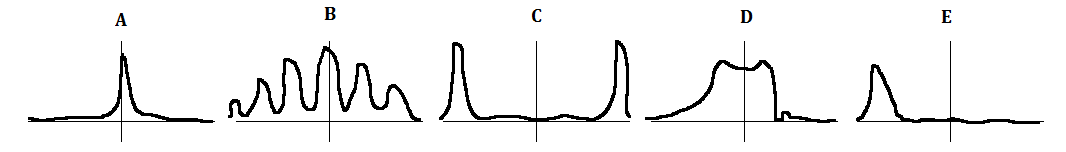
\includegraphics[width=.9\textwidth]{001.png}
	}
\end{figure}


\hqspace

10. You are measuring the length of a fly's foot. Your final result is $l=815nm \pm 1\% $. The most widely accepted experimental value for this particular foot in the literature is $l=821nm \pm 19nm$. The theoretically calculated ideal value is $l=819nm$.

(a) Sketch a graphical depiction of the various results and how they relate.

(b) How far is your mean result from the theoretical value. Express answer three ways: units, number of sigmas, and percentage. What is each of these useful for?

(c) Does the theoretical value lie within a standard deviation of your result?

(d) What is the probability that your result and the literature experiment are mutually consistent, assuming normally distributed uncertainties?












\end{document}